\section{Sekvensdiagrammer}
Sekvensdiagrammerne viser normalforløbene for de givne usecases i kravspecifikationen. På diagrammerne er også vist usecasenes undtagelser og udvidelser. Sekvensdiagrammerne bruges til udviklingen af produktet, hvor kan skabe sig et overblik omkring interaktionen af elementerne på et højere plan. De enkelte blokke svarer til de blokke som er specificeret under block definitions afsnittet: \ref{sub:bdd_hardware}.  

%Dette afsnit består af Sekvensdiagrammer til hver usecase i kravspecifikationen. Et sekvensdiagram fortæller hvilke elementer, som bidrager til det givne forløb og interaktionen i mellem elementerne. I diagrammet er tid vertikalt, hvor der horisontalt sendes beskeder i mellem elementerne. Beskederne kan både være asynkrone(åben pil) og synkrone(udfyldt pil), asynkrone forventer ikke et svar tilbage, hvilket synkron gør. Svaret fra en synkron besked er en stiplet linje. Sekvensdiagrammerne bruges til udviklingen af produktet, hvor kan skabe sig et overblik omkring interaktionen af elementerne på et højere plan.
\subsection{Sekvensdiagram for usecase 1} 
\begin{figure}[H]
	\centering
	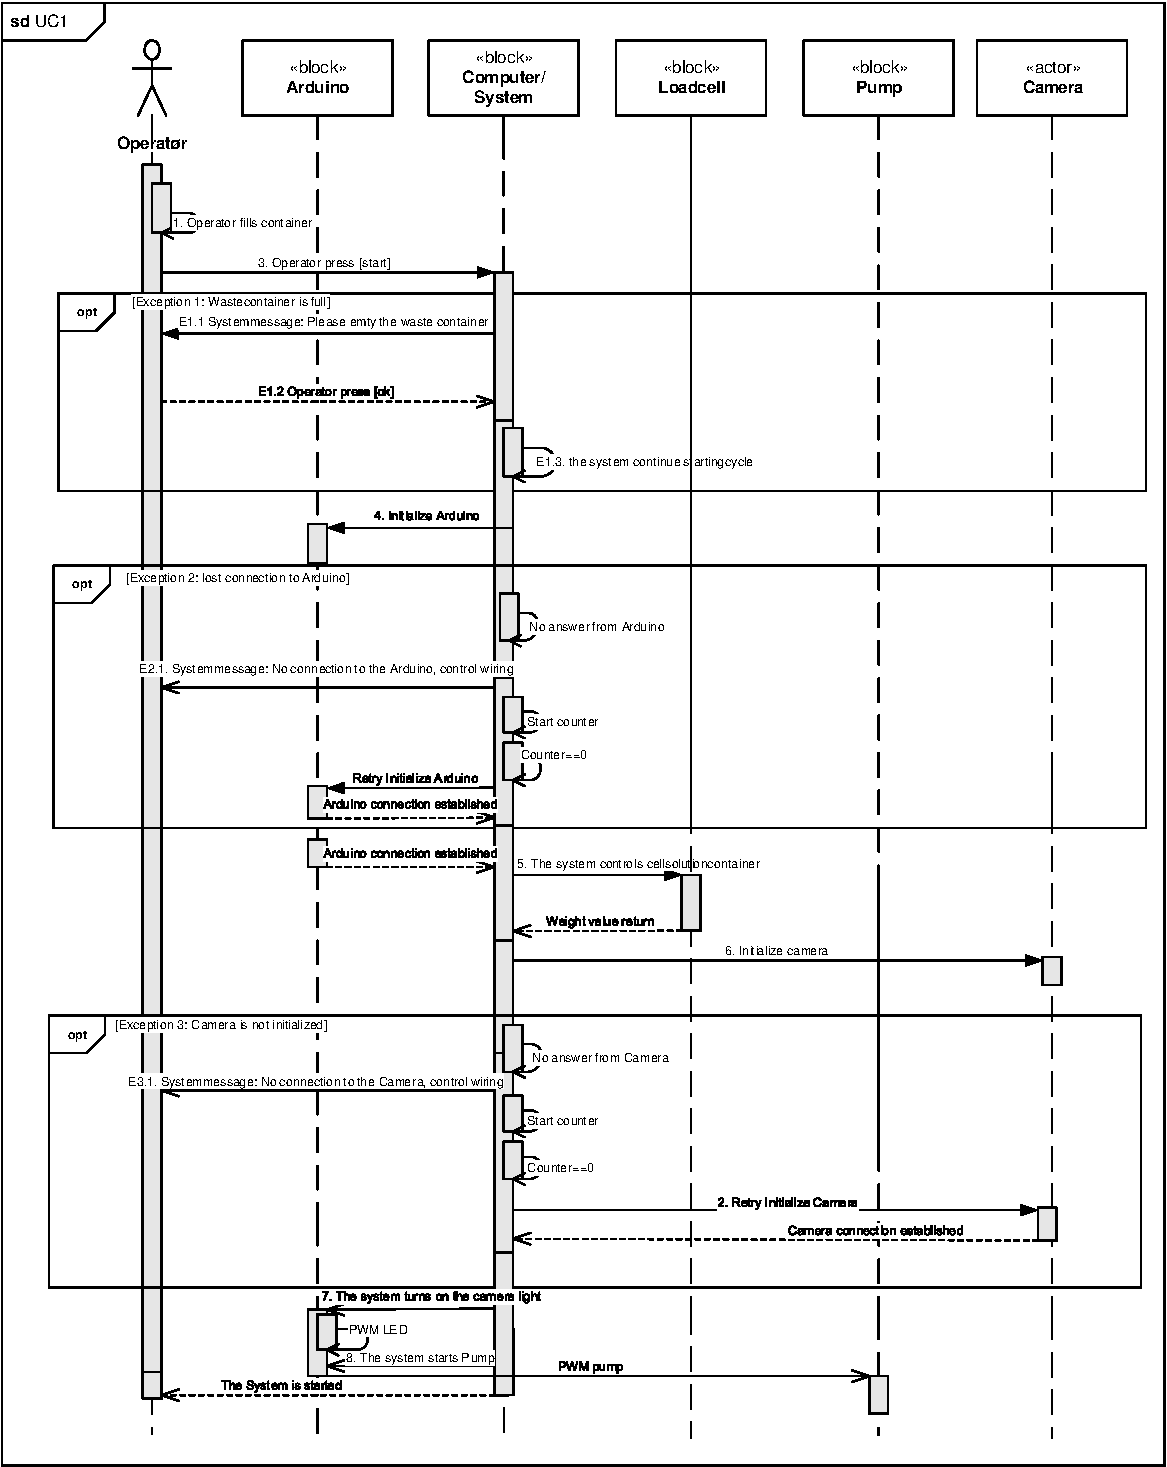
\includegraphics[width=1\textwidth]{pdf/UC1_cropped.pdf}
	\caption{Sekvensdiagram for usecase 1}
	\label{fig:uc1}
\end{figure}

\subsection{Sekvensdiagram for usecase 2} 
\begin{figure}[H]
	\centering
	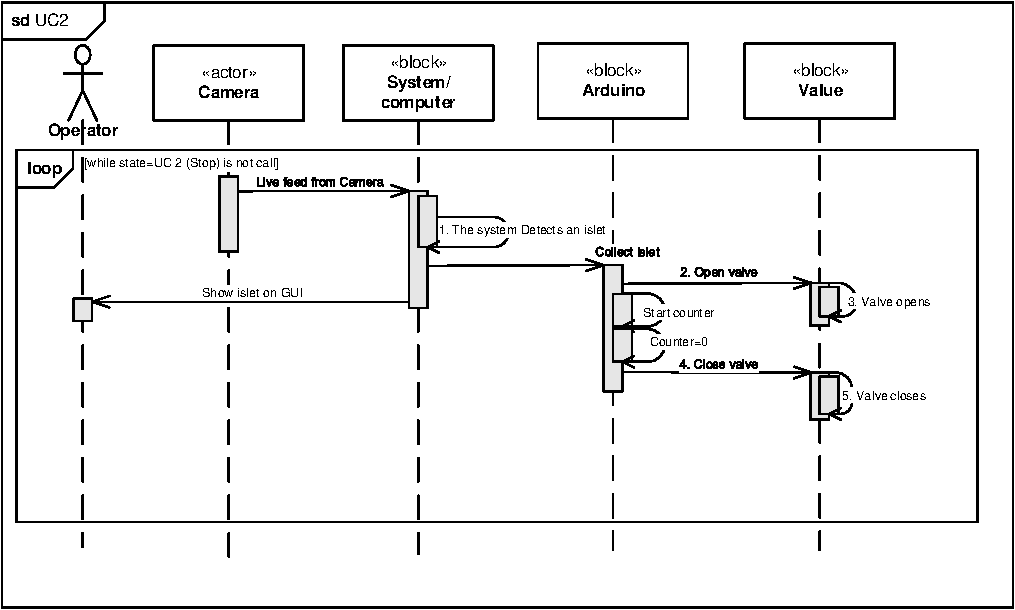
\includegraphics[width=1\textwidth]{pdf/UC2_cropped.pdf}
	\caption{Sekvensdiagram for usecase 2}
	\label{fig:uc1}
\end{figure}

\subsection{Sekvensdiagram for usecase 3} 
\begin{figure}[H]
	\centering
	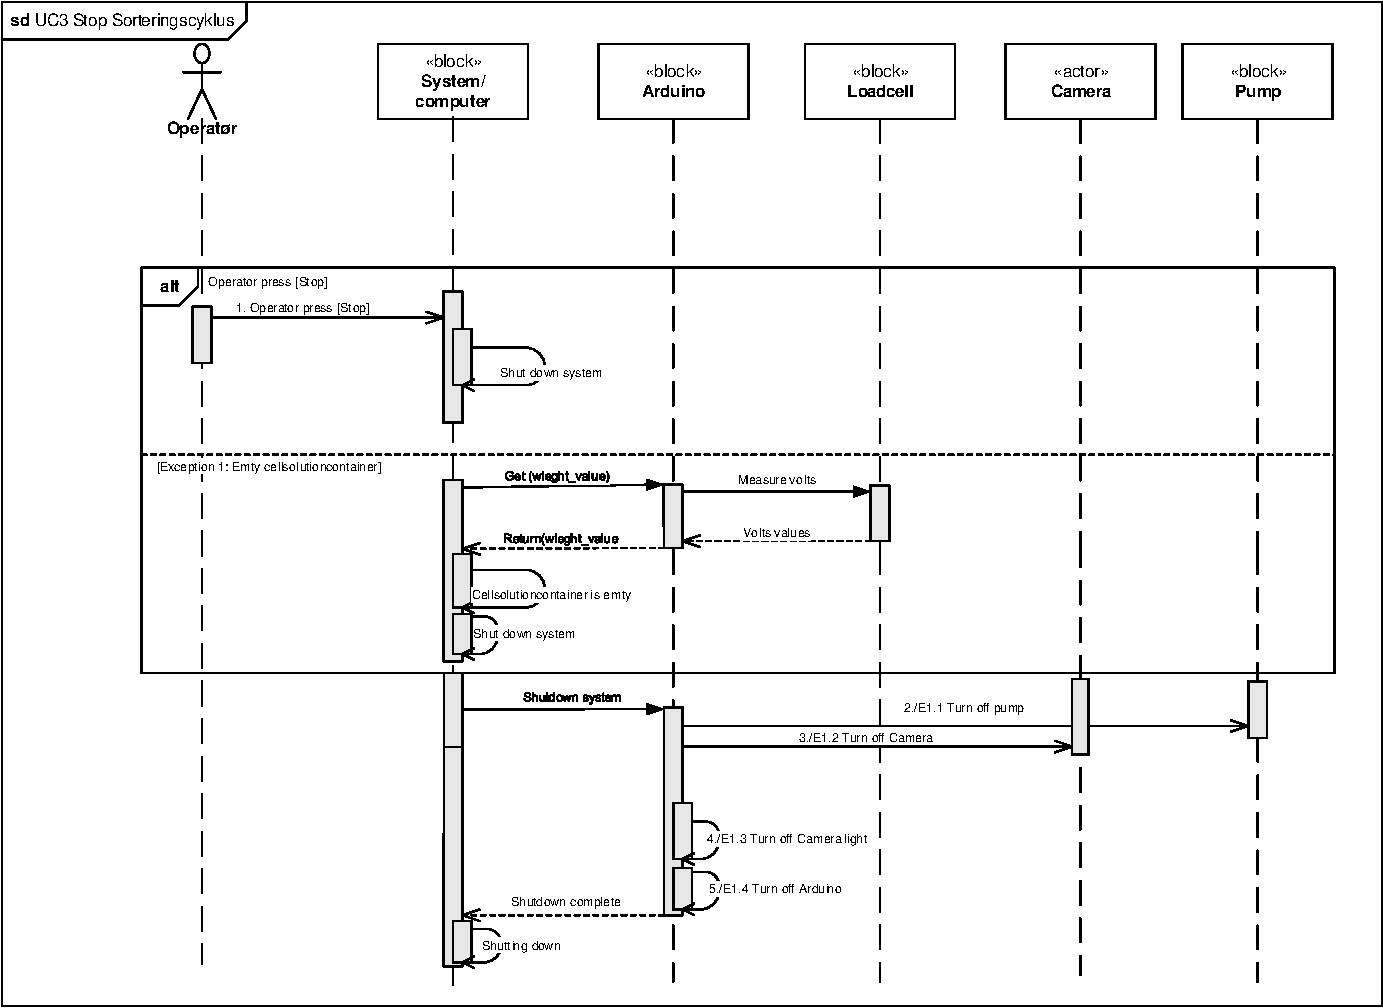
\includegraphics[width=1\textwidth]{pdf/UC3_cropped.pdf}
	\caption{Sekvensdiagram for usecase 3}
	\label{fig:uc1}
\end{figure}

\subsection{Sekvensdiagram for usecase 4} 
\begin{figure}[H]
	\centering
	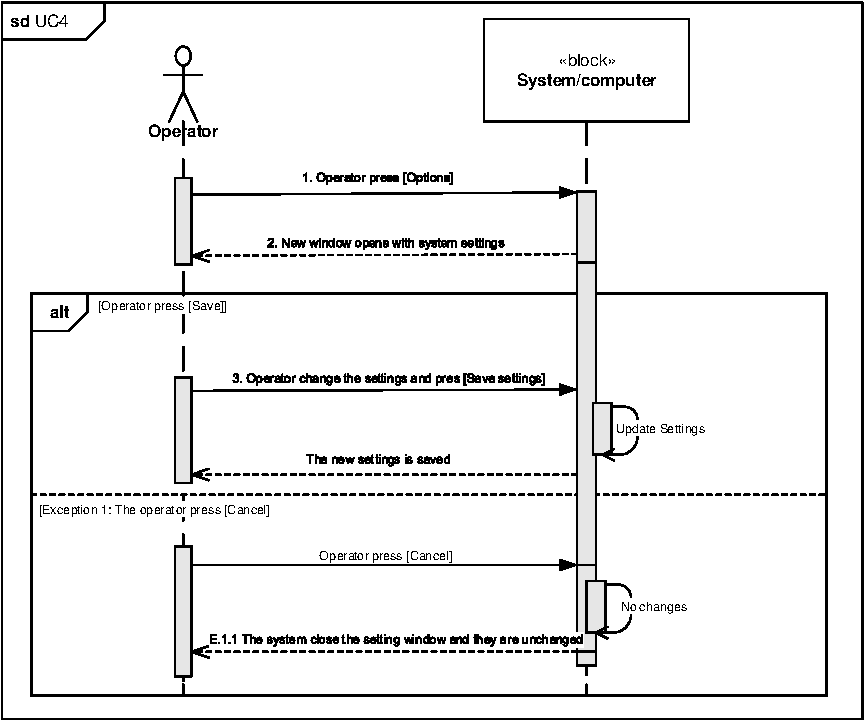
\includegraphics[width=1\textwidth]{pdf/UC4_cropped.pdf}
	\caption{Sekvensdiagram for usecase 4}
	\label{fig:uc1}
\end{figure}

\subsection{Sekvensdiagram for usecase 5} 
\begin{figure}[H]
	\centering
	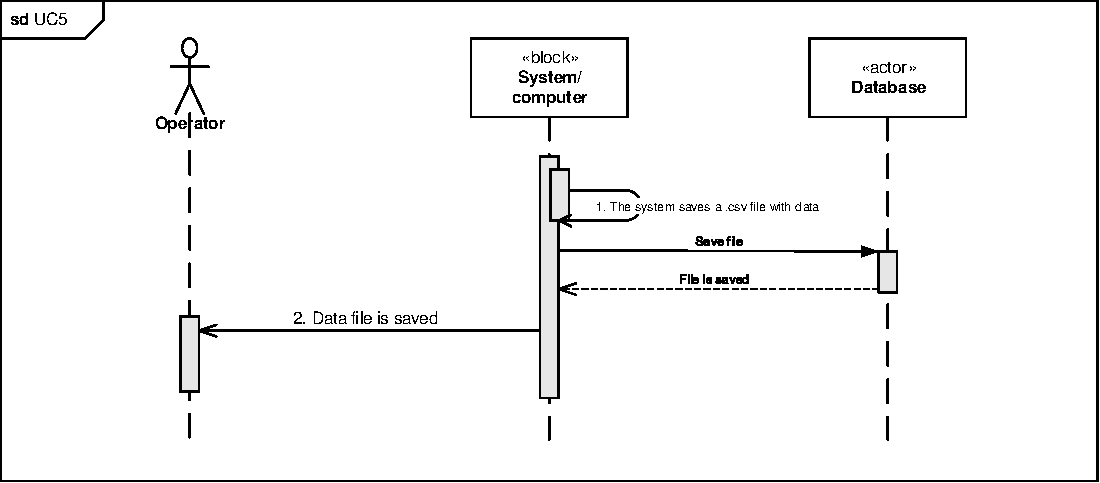
\includegraphics[width=1\textwidth]{pdf/UC5_cropped.pdf}
	\caption{Sekvensdiagram for usecase 5}
	\label{fig:uc1}
\end{figure}
